\newpage
\section{Vorbereitung}

    \subsection{Begriffserklärung}

        \subsubsection{Switch-Stacking}

        Switch-Stacking ist ein wichtiges Merkmal von Netzwerk-Switches.
        Diese Switches können miteinander verbunden werden, um als 
        logische Einheit zu fungieren. Durch das Zusammenschalten weiterer Switche, wird die Netzwerkkapazität 
        dank der höheren Anzahl verfügbarer Ports, besserer Ausfallsicherheit und der Möglichkeit 
        Link-Aggregation zu betreiben, erheblich erhöht. 
        Switch-Stacking wird nur von stapelbaren Switches unterstützt. \\\\
        Switches in einem Stack können mittels DAC-Kabeln, optischen Transceiver oder Stacking-Kabeln verbunden werden. 
        Es gibt einen Stack-Master, der das Zentrum des Stack-Systems ist und die Konfigurationsdaten verwaltet. 
        Die anderen Switches im Stack werden als Stack-Slaves bezeichnet. 
        Der Stack-Master kann von Benutzern verwaltet werden, und falls er ausfällt, wird ein neuer Master-Switch unter den Slaves ausgewählt.\\\\
        Zusammenfassend lassen sich folgende Vorteile von Switch-Stacking erschließen:
        \begin{itemize}
            \item Verbesserung der Zuverlässigkeit und Flexibilität des Netzwerkes
            \item Erhöhung der Bandbreite und Vereinfachung der Vernetzung
            \item hohe Skalierbarkeit des Netzwerkes
        \end{itemize}

        \subsubsection{Switchkaskadierung}

        Kaskadierung ist die traditionelle Methode zum Verbinden mehrerer Ethernet-Switches 
        und umfasst verschiedene Methoden für unterschiedliche Netzwerktopologien.\\
        Durch die Verknüpfung mehrerer Switches können Benutzer mehrere Ports haben, 
        die jeden Switch miteinander verbinden, unabhängig voneinander konfiguriert 
        und als Gruppe verwaltet werden können. 
        In einem Kaskaden-Switch-Netzwerk sind Daisy-Chain-Topologie und 
        Sterntopologie zwei gängige Methoden. 

        \subsubsection{Spanning-Tree-Verfahren}

        Der Spanning-Tree-Algorithmus führt eine Reihe von Schritten aus, 
        um sicherzustellen, dass die Topologie schleifenfrei ist und das Ethernet ordnungsgemäß funktioniert:\\
        \begin{enumerate}
            \item Root-Bridge-Auswahl – Zuerst wählt STP eine Root-Bridge aus. Dies ist der wichtigste Schalter in der Topologie. Es ist die Wurzel des azyklischen Baums.
            \item Schleifentopologie-Erkennung – Sobald die Root-Bridge ausgewählt ist, beginnt sie mit dem Senden von Spanning-Tree-Nachrichten (BPDUs). Der Switch verwendet diese Nachrichten, um den Teil der Topologie zu finden, der die Schleife enthält.
            \item Bestimmen der Port-Rollen – Nach dem Bestimmen des Loop-Teils der Topologie platziert jeder Switch so viele Switch-Ports wie nötig, um sicherzustellen, dass die Topologie schleifenfrei ist.
            \item Dropout – Switches tauschen weiterhin Nachrichten aus, um die Verfügbarkeit von Links und Nachbarkontakten zu verfolgen. Wenn die Verbindung oder der Switch ausfällt, führt der Switch die Schritte 2 und 3 erneut aus, um sicherzustellen, dass die neue Topologie schleifenfrei ist.
        \end{enumerate}

        \subsubsection{Auto-Negoatiation}

        Auto-Negotiation ist eine Funktion, die es zwei Netzwerken mit unterschiedlichen Geschwindigkeiten
        ermöglicht, zu kommunizieren und sich an eine Geschwindigkeit anpasst, 
        die für beide Netzwerke geeignet ist. 
        Beispielsweise verfügt ein Switch über einen 1-Gbit/s-Port (Gigabit-Ethernet), 
        der mit einem 100-Mbit/s-Port (Fast Ethernet) an einem anderen Switch verbunden ist. 
        Die Portgeschwindigkeiten an beiden Enden müssen gleich sein, um eine Verbindung herzustellen. 
        Das Autonegotiation-Protokoll teilt Baudrate, Duplexmodusstatus und Flusssteuerungsinformationen zwischen zwei Ports. 
        Sobald der Port die obigen Parameterinformationen empfangen hat, 
        passt er seinen Pegel entsprechend den Fähigkeiten des Peer-Ports an.

        \subsubsection{AutoUplink(MDI/MDI-X)}

        Ein Ethernet-Netzwerkport (z. B. an einem Switch) verwendet die automatische Uplink-Funktion, um zu erkennen, 
        an welchen Switch er senden und empfangen (MDI/MDIX) soll. 
        Mit der automatischen Uplink-Funktion können sowohl Crossover-Kabel 
        als auch 1:1-Netzwerkkabel verwendet werden.

        \subsubsection{Link Aggregation/ Port Trunking}
        Link Aggregation ist eine Methode zur Zusammenfassung mehrerer Netzwerkverbindungen 
        zu einer logischen Verbindung. Clustering erhöht den Datendurchsatz und reduziert Fehler. 
        Standardisiert ist das Verfahren im IEEE-Standard 802.1AX, der 2008 den älteren Standard 
        802.3ad ablöste. Neben diesen Standards gibt es auch herstellerspezifische Implementierungen.

        \begin{quote}
            ``Port Trunking ist das Zusammenfassung der Verbindungen mehrerer physischer Ports zu einer 
            logischen Verbindung höherer Bandbreite.`` \cite*{portTrunking}
        \end{quote}
        Eine Trunk-Leitung kombiniert logisch oder physisch mehrere Kommunikationsverbindungen oder -kanäle zu 
        einer einzigen Leitung oder logischen Verbindung. Diese angeschlossenen Leitungen werden in 
        vielen verschiedenen Bereichen der Netzwerk- und Kommunikationstechnik, wie beispielsweise 
        Switches, Telefonanlagen oder anderen Netzwerkkomponenten eingesetzt.

        \subsubsection{Vollduplex-Betrieb}
        In der Kommunikationstechnik bezeichnet Duplex (Vollduplex), Halbduplex oder Simplex die 
        Richtwirkung des Kommunikationskanals.
        \begin{itemize}
            \item Simplex (SX) ist ein Richtungsbetrieb. Das bedeutet, dass Informationen nur in eine bestimmte Richtung übertragen werden (nur Nachrichten senden oder empfangen), z.B. Radio, TV oder Pager
            \item Halbduplex (HX), ist ein Zwei-Wege-Betrieb. Informationen können in beide Richtungen fließen, aber nicht gleichzeitig, z.B. Funkamateur
            \item Vollduplex (DX, manchmal FDX) ist ein synchroner Betrieb. Dadurch können Informationen gleichzeitig in beide Richtungen übertragen werden, z.B. Telefon
        \end{itemize}

        \newpage
        \subsubsection{Mac-Adressenfilter}
        Ein MAC-Filter (MAC-Adressfilter) ist ein Netzwerkzugriffsschutz, 
        der nur Geräten mit bestimmten MAC-Adressen den Zugriff auf das Netzwerk 
        ermöglicht. MAC-Filter werden üblicherweise im LAN oder WLAN verwendet und 
        sind als Tabelle im Router (Firewall) hinterlegt. Aus Sicherheitsgründen ist 
        der MAC-Filter jedoch ein schwacher Zugriffsschutz, da er leicht umgangen werden kann.

    \newpage
    \subsection{Netzwerktrennung}

        \subsubsection{VLAN}
        Die Virtual LAN (VLAN)-Technologie ermöglicht es Netzwerkadministratoren, 
        die logische Netzwerkkonnektivität von der physischen Konnektivität zu trennen. 
        Dieses Konzept unterscheidet sich von einem herkömmlichen LAN insofern, als ein LAN 
        durch seine physische Konnektivität begrenzt ist. Alle Benutzer in einem LAN gehören 
        zu einer einzigen Broadcast-Domäne1 und können auf der Datenverbindungsschicht oder 
        "Schicht 2" miteinander kommunizieren. Netzwerkmanager haben LANs verwendet, um ein 
        komplexes Netzwerk in kleinere Einheiten aufzuteilen, um es besser verwalten zu können 
        und die Leistung und Sicherheit zu verbessern. Zum Beispiel verwenden Netzwerkmanager 
        ein LAN für jedes IP-Subnetz in ihrem Netzwerk. Die Kommunikation zwischen den Subnetzen 
        wird auf der Netzwerkschicht oder "Schicht 3" durch IP-Router ermöglicht.\\
        Ein VLAN kann man sich als ein einziges physisches Netzwerk vorstellen, das logisch in 
        einzelne LANs unterteilt werden kann, die unabhängig voneinander arbeiten können.

        \begin{figure}[ht]
            \centering
            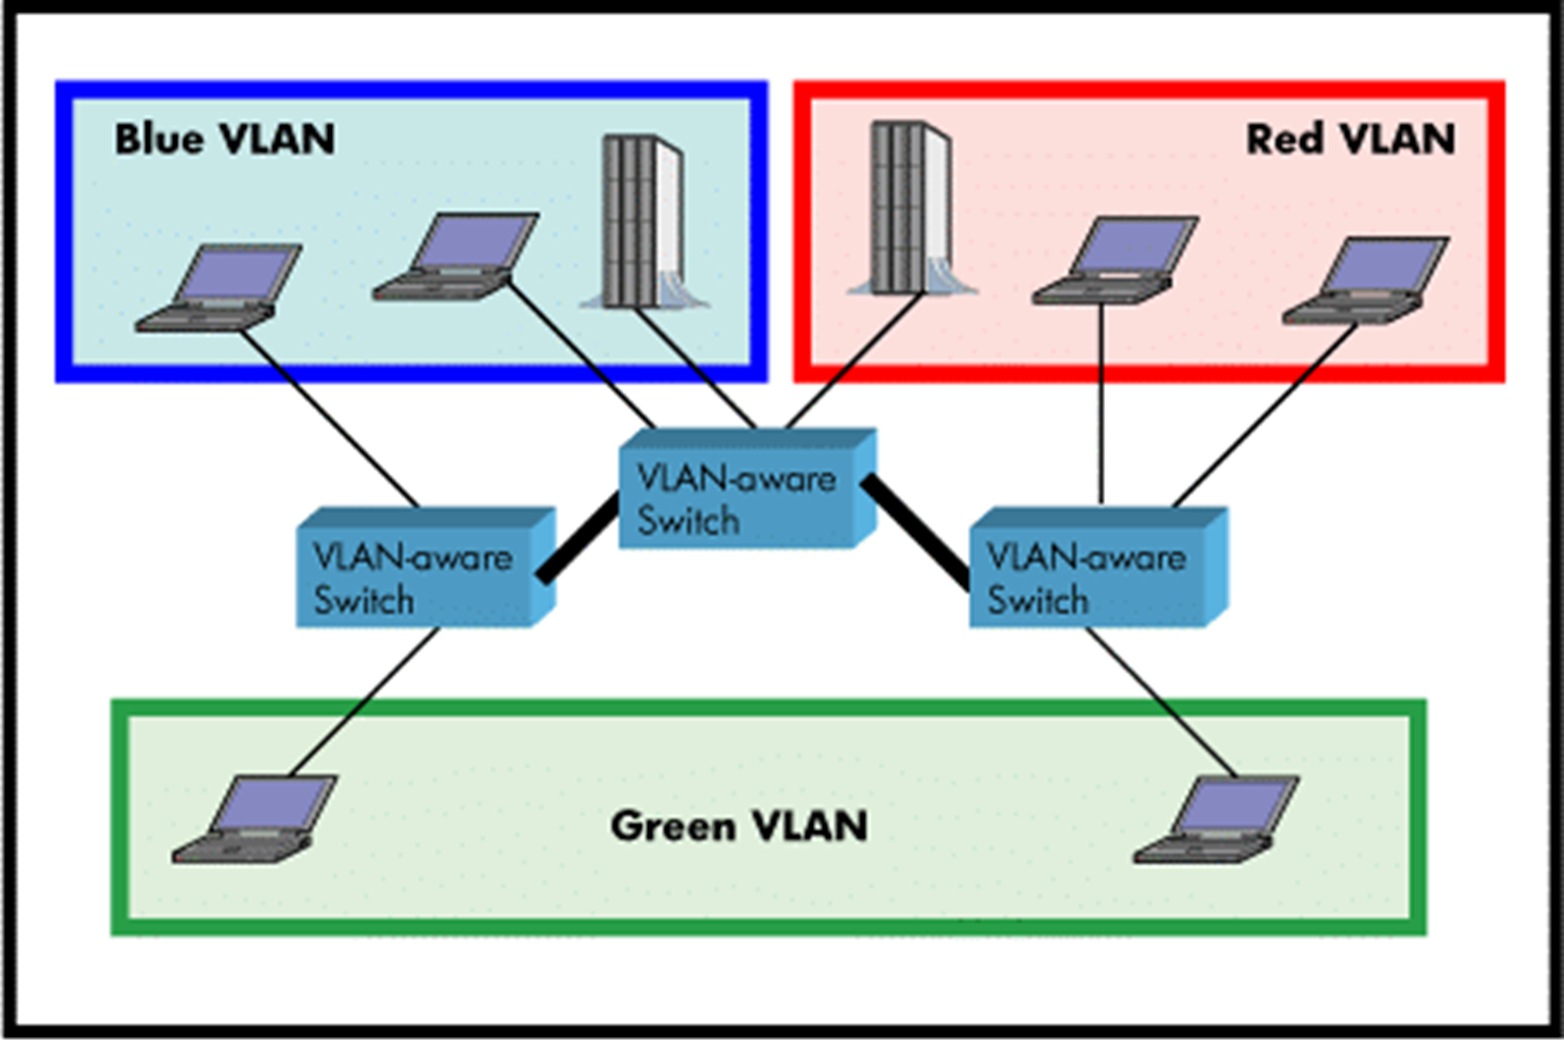
\includegraphics{images/VLAN.png}
            \caption{Verwenden von VLANs zum Erstellen unabhängiger Broadcast-Domänen über Switches hinweg}
        \end{figure}
        Abbildung 1 verdeutlicht einige wesentliche Unterschiede zwischen herkömmlichen LANs und VLANs.
        \begin{itemize}
            \item Alle Switches sind miteinander verbunden. Es gibt jedoch drei verschiedene VLANs oder Broadcast-Domänen im Netz. Eine physische Isolierung ist für die Definition von Broadcast-Domänen nicht erforderlich. Wenn Abbildung 1 ein herkömmliches LAN ohne VLAN-fähige Switches wäre, würden alle Stationen zu einer Broadcast-Domäne gehören.
            \item Alle Switch-Ports können auf der Datenübertragungsschicht miteinander kommunizieren, wenn sie Mitglieder desselben VLAN werden.
            \item Der physische Standort einer Endstation definiert nicht ihre LAN-Grenze.
            \begin{itemize}
                \item Eine Endstation kann physisch von einem Switch-Port zu einem anderen verschoben werden, ohne ihre "Sicht auf das Netzwerk" zu verlieren. Das heißt, die Menge der Stationen, mit denen sie auf der Datenübertragungsschicht kommunizieren kann, bleibt dieselbe, vorausgesetzt, dass ihre VLAN-Mitgliedschaft ebenfalls von Port zu Port migriert wird.
                \item Durch die Neukonfiguration der VLAN-Mitgliedschaft des Switch-Ports, an den eine Endstation angeschlossen ist, können Sie die Netzwerkansicht der Endstation einfach ändern, ohne dass ein physischer Wechsel von Port zu Port erforderlich ist.
            \end{itemize}
        \end{itemize}

        \subsection{Vorteile von VLAN}
        Zu den wichtigsten Vorteilen der Verwendung von VLANs gehören die folgenden:
        \begin{itemize}
            \item Bandbreitenerhalt: Ein gut konzipiertes VLAN trägt dazu bei, den Broadcast- und Multicast-Verkehr auf die Stationen zu beschränken, die den mit diesem VLAN verbundenen Verkehr hören und darauf reagieren. Die Netzwerk- und Computerressourcen von nicht teilnehmenden Stationen werden nicht beeinträchtigt, wodurch die Leistung verbessert wird.
            \item Verwaltbarkeit: Umzüge, Hinzufügungen und Änderungen der Netzwerktopologie erfordern keine physischen Änderungen der Netzwerktopologie. Die Mobilität der Benutzer ist aufgrund der dynamischen Natur von VLANs viel einfacher. Physikalisch verteilte Arbeitsgruppen können logisch innerhalb derselben Broadcast-Domäne verbunden werden, so dass es so aussieht, als befänden sie sich im selben physischen LAN. Eine einzige physische Verbindung kann gleichzeitig mehrere IP-Subnetze bedienen, wenn subnetzbasierte VLANs auf dieser Verbindung konfiguriert sind. Endstationen, die VLANs verwenden, können lokal rudimentäre Class of Service (CoS) anbieten, indem sie dem Datenverkehr für bestimmte Aktivitäten Priorität einräumen.
            \item Verbesserte Sicherheit: Sie können verschiedene Sicherheitsdomänen einrichten, um verschiedene Sicherheitsstufen im Netzwerk bereitzustellen, da das Netzwerkdesign flexibler ist als das von herkömmlichen LANs. Da Frames nur dann an einen Zielport weitergeleitet werden, wenn der Port zum selben VLAN wie der Frame gehört, tragen VLANs dazu bei, die Isolierung des Datenverkehrs zu erzwingen, und bieten so eine zusätzliche Sicherheitsebene im Netzwerk.
        \end{itemize}

        \subsection{VLAN-fähige Switches sind der Schlüssel}

        \subsubsection{VLAN-Tagging}
        Wie bereits erwähnt, können Sie die VLAN-Funktionalität durch explizites Frame-Tagging 
        durch Switches und Endstationen implementieren. Netzwerk-Switches und -Endstationen, die 
        über VLANs Bescheid wissen, werden als VLAN-bewusst bezeichnet. Netzwerk-Switches und -Endstationen, die VLAN-Tags interpretieren können, werden als VLAN-Tag-fähig bezeichnet. VLAN-Tag-fähige Switches und Endstationen fügen VLAN-Tags zu Standard-Ethernet-Frames hinzu - ein Prozess, der explizites Tagging genannt wird. Beim expliziten Tagging bestimmt die Endstation oder der Switch die VLAN-Zugehörigkeit eines Frames und fügt ein VLAN-Tag in den Frame-Header ein (siehe Abbildung 2), so dass nachgelagerte Link-Partner nur das Tag untersuchen können, um die VLAN-Zugehörigkeit zu bestimmen.
        Das Tagging hat mehrere Vorteile: Die VLAN-Zuordnung muss nur einmal an einer Endstation oder an einem Edge-Switch vorgenommen werden, so dass die nachgeschalteten Switches auf dem gesamten Weg zum Ziel von der Klassifizierung der Frames entlastet werden. Das Tagging an Endstationen ist besonders vorteilhaft, da der Overhead der Rahmenklassifizierung verteilt wird.


    \newpage
    \subsection{Übersicht des NETGEAR-Switches}